
\documentclass{bredelebeamer}

% Amélie : Environnement, SSLstrip et conclusion
% Brendan : intro HTTP, HTTPS interception
% Simon : état de l'art, SSLStrip+ et SSLStrip-NTP


%%%%%%%%%%%%%%%%%%%%%%%%%%%%%%%%%%%%%%%%%%%%%%%%

\title[Attaques sur connexions HTTPS]{Attaques man-in-the-middle de HTTPS}
\subtitle{SSLStrip, HTTPS-Interception...}
\author[S. Duret - A. Risi - B. Guevel]{Simon Duret \\ Amélie Risi \\ Brendan Guevel}
\institute[]{
  
\includegraphics[scale=0.2]{../medias/universite-bordeaux.pdf}
}

\date{14 mai 2018}

%%%%%%%%%%%%%%%%%%%%%%%%%%%%%%%%%%%%%%%%%%%%%%%%%%%%%%%%%%%%%%%%%%%%%


\begin{document}

%%%%%%%%%%%%%%%%%%%%%%%%%%%
% Titre                   %
%%%%%%%%%%%%%%%%%%%%%%%%%%%
\begin{frame}
  \titlepage
\end{frame}

%%%%%%%%%%%%%%%%%%%%%%%%%%%
% Introduction            %
%%%%%%%%%%%%%%%%%%%%%%%%%%%
\begin{frame}{Introduction}

  {\Large \centerline{HTTP est \emph{le} protocole central du net}}
  \hspace{40cm}

  \begin{columns}
    \begin{column}{0.5\textwidth}
      \begin{itemize}
        % Dire à l'oral que client = navigateur généralement, et serveur = site web
      \item{Assure la transmission des données}
      \item{Architecture client/serveur}
      \end{itemize}
      \begin{alertblock}{Problème}
        \begin{itemize}
        % Donner des exemples à l'oral : interception du wifi, ou physiquement au niveau du cable ethernet, ...
        \item{Tout le trafic est en clair}
        \end{itemize}
      \end{alertblock}

      \begin{exampleblock}{Solution}
        \begin{itemize}
        \item{HTTPS : extension de HTTP}
          % (mot de passe, numéro de carte bancaire, ...)
        \item{Confidentialité et authentification}
        \end{itemize}
      \end{exampleblock}
    \end{column}
    \begin{column}{0.5\textwidth}
      
\includegraphics[width=\linewidth]{../medias/www.png}
    \end{column}
  \end{columns}

  \hspace{20cm}

  {\Large \centerline{Malgré cette protection, des attaques restent possibles...}}


\end{frame}


%%%%%%%%%%%%%%%%%%%%%%%%%%
%  Plan                  %
%%%%%%%%%%%%%%%%%%%%%%%%%%
\begin{frame}{Plan}
  \tableofcontents
\end{frame}


\section{Fonctionnement de HTTP/HTTPS}

%%%%%%%%%%%%%%%%%%%%%%%%%%%
%  Fonctionnement de HTTP %
%%%%%%%%%%%%%%%%%%%%%%%%%%%

\begin{frame}{Fonctionnement de HTTP}
    \begin{columns}
        \begin{column}{0.5\textwidth}
            \begin{block}{Protocole client-serveur}
                \begin{itemize}
                    \item{Client : requête HTTP}
                    \item{Serveur : envoi de la ressource}
                \end{itemize}
            \end{block}
        \end{column}

        \begin{column}{0.5\textwidth}
            \begin{exampleblock}{Navigateur web}
                \begin{itemize}
                    \item{Rend le processus transparent}
                    \item{Met en forme le html/css}
                \end{itemize}
            \end{exampleblock}
        \end{column}
    \end{columns}

    \hspace{40cm}

    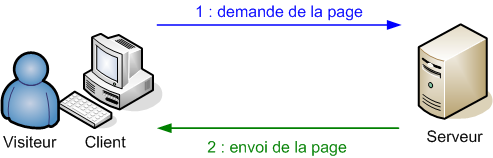
\includegraphics[width=\linewidth]{../medias/requete-http.png}
\end{frame}

%%%%%%%%%%%%%%%%%%%%%%%%%%%
%  Exemple de HTTP        %
%%%%%%%%%%%%%%%%%%%%%%%%%%%

\begin{frame}{Exemple d'une requête HTTP}
    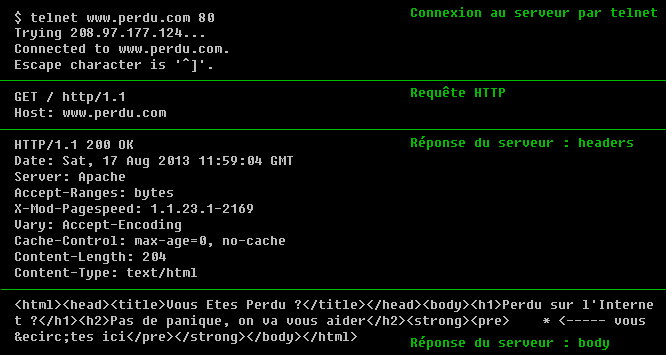
\includegraphics[width=\linewidth]{../medias/perdu.png}
    % Faire une petite démo en live (avec la même requête)
\end{frame}

%%%%%%%%%%%%%%%%%%%%%%%%%%%
%  HTTPS                  %
%%%%%%%%%%%%%%%%%%%%%%%%%%%

\begin{frame}{HTTPS : la version chiffrée de HTTP}
    
\includegraphics[width=\linewidth]{../medias/http-ssl.png}

    \hspace{10cm}

    % Dire à l'oral **qu'on ne touche pas à HTTP** et qu'on rajoute simplement le chiffrement par dessus
    \begin{columns}
        \begin{column}{0.5\textwidth}
            \begin{exampleblock}{Protocole SSL/TLS}
                \begin{itemize}
                    \item{Authentification du serveur}
                    \item{Confidentialité des données}
                    \item{Intégrité des données}
                \end{itemize}
            \end{exampleblock}
        \end{column}

        \begin{column}{0.5\textwidth}
            \begin{block}{Utilisé pour}
                \begin{itemize}
                    \item{Navigation web : HTTPS}
                    \item{Protocole mail : SMTPS}
                    \item{VPN : OpenVPN}
                \end{itemize}
            \end{block}
        \end{column}
    \end{columns}
    \hspace{20cm}

    {\Large \centerline{\alert{Limitation} : IP/port de destination toujours visible (pour routage)}}
\end{frame}


%%%%%%%%%%%%%%%%%%%%%%%%%%%
%  Certificats            %
%%%%%%%%%%%%%%%%%%%%%%%%%%%

\begin{frame}{Gestion des certificats}
    % Permet d'authentifier la communication \\
    % Sur internet, cela sert essentiellement à s'assurer de l'identité du serveur \\
    % Nécessité d'une authorité de certification (un tiers) \\
    \includegraphics[width=\linewidth]{../medias/autorite-certification.png}
\end{frame}

%%%%%%%%%%%%%%%%%%%%%%%%%%%
%  TLS                    %
%%%%%%%%%%%%%%%%%%%%%%%%%%%

\begin{frame}{Le protocole SSL/TLS}
    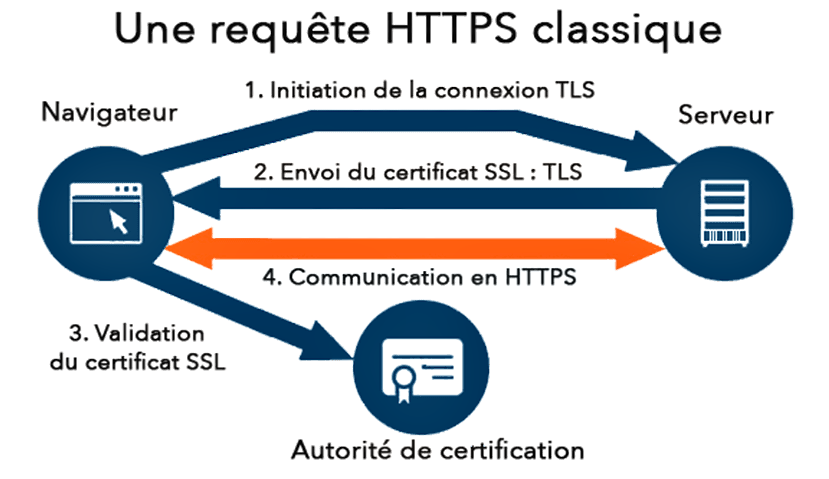
\includegraphics[width=\linewidth]{../medias/protocole-tls.png}
\end{frame}


\section{Etat de l'art des attaques sur HTTPS}

%%%%%%%%%%%%%%%%%%%%%%%%%%%
%  Attaques HTTPS         %
%%%%%%%%%%%%%%%%%%%%%%%%%%%

\begin{frame}{Attaques sur HTTPS}

  {\Large \centerline{Plusieurs angles d'attaques :}}

  \begin{columns}
    \begin{column}{0.5\textwidth}
      \begin{exampleblock}{Failles d'implémentation}
        \begin{itemize}
        \item Bibliothèques (openssl)
        \item Navigateurs (Internet Explorer)
        \end{itemize}
      \end{exampleblock}

      \begin{exampleblock}{Cryptographie}
        \begin{itemize}
        \item Mode de chiffrement (CBC)
        \item Algorithmes (RC4)
        \end{itemize}
      \end{exampleblock}

      \begin{exampleblock}{Protocole}
        \begin{itemize}
        \item{Downgrade attack}
        \item{SSLv3 (POODLE)}
        \end{itemize}
      \end{exampleblock}
    \end{column}

    \begin{column}{0.5\textwidth}
      \begin{figure}
        
\includegraphics[width=0.32\linewidth]{../medias/heartbleed.png}
      \end{figure}
      \begin{figure}
        
\includegraphics[width=0.32\linewidth]{../medias/sweet32.png}
      \end{figure}
      \begin{figure}
        
\includegraphics[width=0.32\linewidth]{../medias/poodle.png}
      \end{figure}
    \end{column}
  \end{columns}

\end{frame}

%%%%%%%%%%%%%%%%%%%%%%%%%%%
%  Historique SSL/TLS     %
%%%%%%%%%%%%%%%%%%%%%%%%%%%

\begin{frame}{Historique des attaques sur SSL/TLS}
    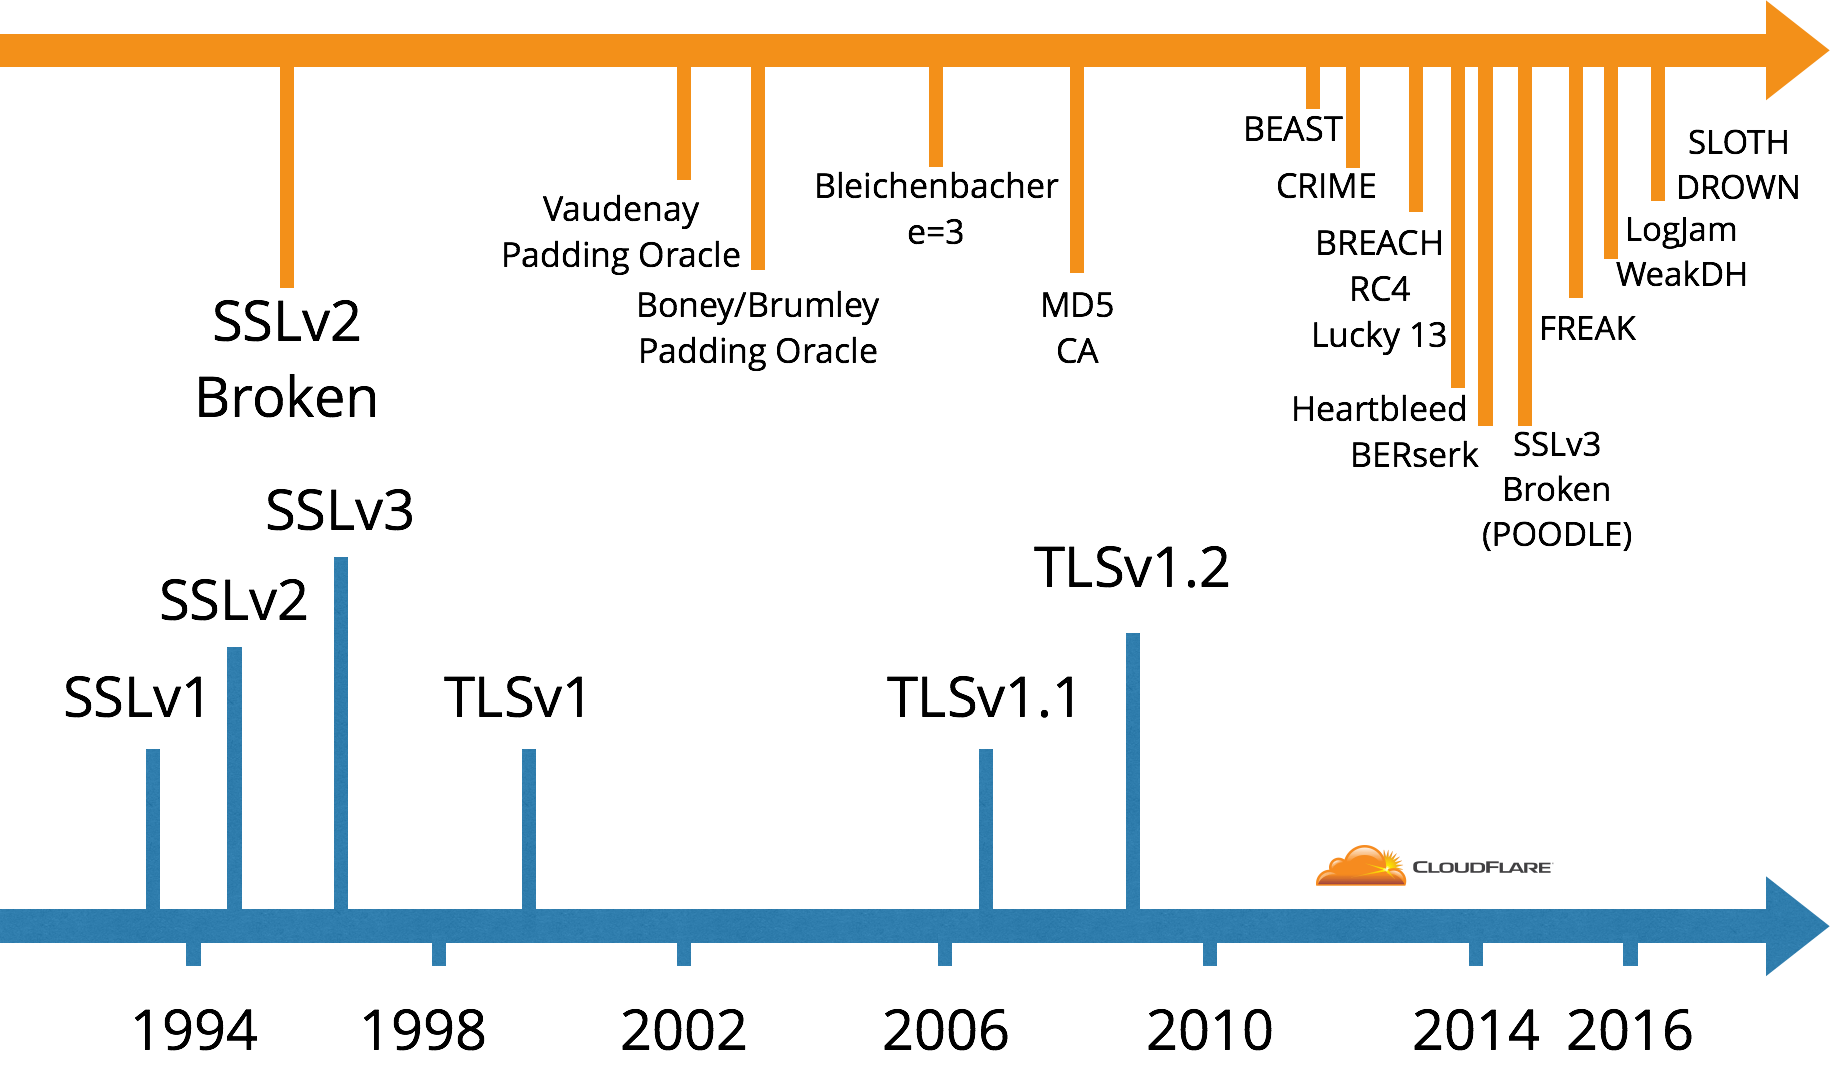
\includegraphics[width=\linewidth]{../medias/history-tls-attacks.png}
\end{frame}


\section{Environnement de nos attaques}

%%%%%%%%%%%%%%%%%%%%%%%%%%%
%  Environnement          %
%%%%%%%%%%%%%%%%%%%%%%%%%%%

\begin{frame}[fragile]{Environnement de nos attaques}
  \begin{columns}
    \begin{column}{0.5\textwidth}
      \begin{block}{Qemunet}
        \begin{itemize}
        \item Outil pour créer un réseau virtuel
        \item \url{gitlab.inria.fr/esnard/qemunet}
        \end{itemize}
      \end{block}

      \begin{exampleblock}{3 machines}
        \begin{itemize}
        \item Un client (Alpine)
        \item Un serveur (Debian)
        \item Un attaquant (Debian)
        \end{itemize}
      \end{exampleblock}

      \begin{exampleblock}{Lancement de l'attaque SSLStrip}
        \verb+./qemunet/qemunet.sh -x -S sslstrip+

      \end{exampleblock}

    \end{column}

    \begin{column}{0.5\textwidth}
      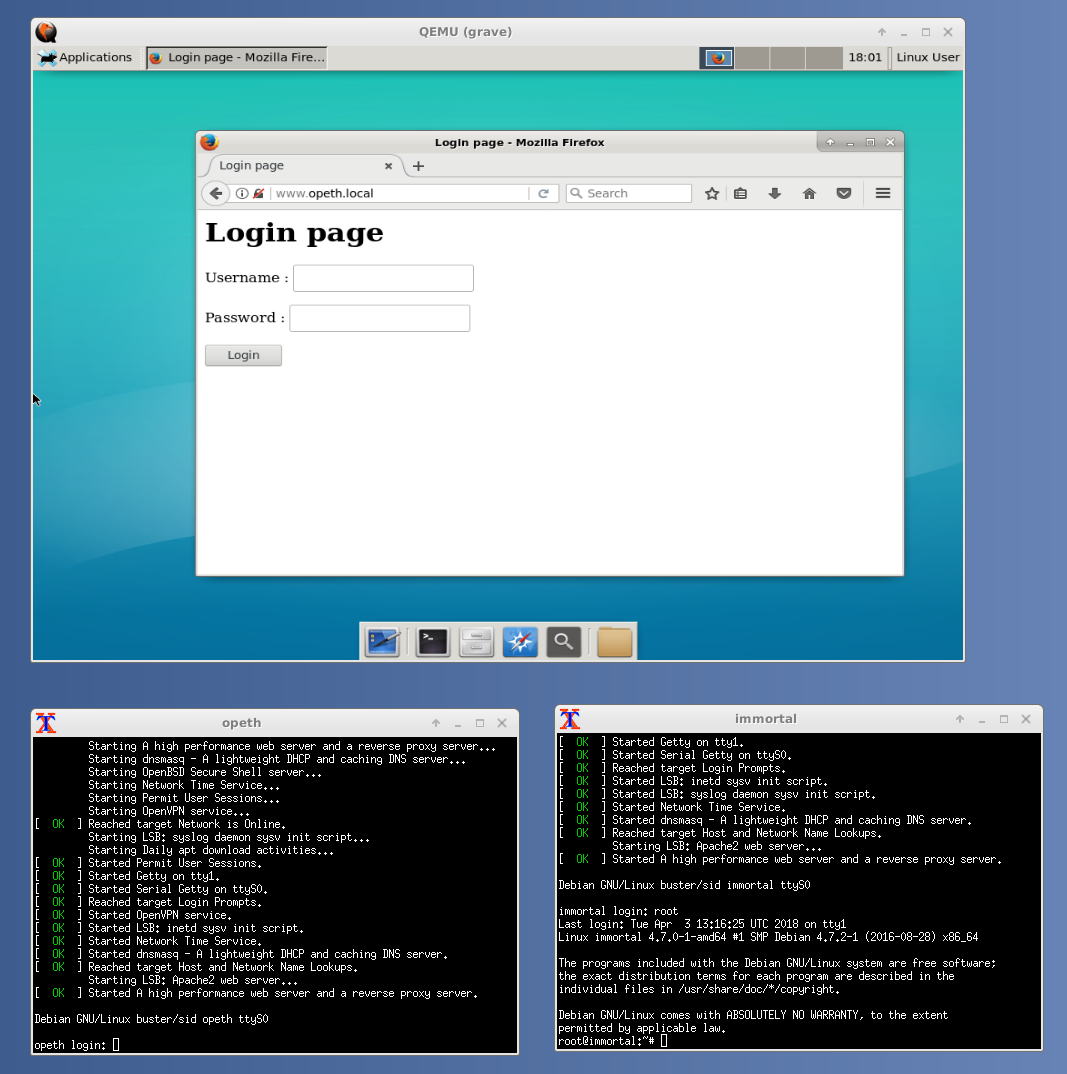
\includegraphics[width=\linewidth]{../medias/qemunet.png}
    \end{column}
  \end{columns}

\end{frame}

%%%%%%%%%%%%%%%%%%%%%%%%%%%
%  Topologie              %
%%%%%%%%%%%%%%%%%%%%%%%%%%%

\begin{frame}{Topologie}
    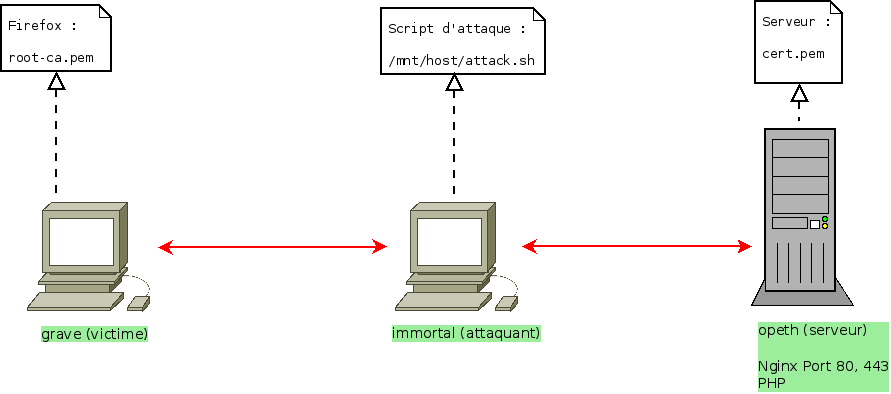
\includegraphics[width=\linewidth]{../medias/topology.png}
\end{frame}


\section{SSLStrip}

%%%%%%%%%%%%%%%%%%%%%%%%%%%
%  Principes              %
%%%%%%%%%%%%%%%%%%%%%%%%%%%

\begin{frame}[fragile]{Attaque SSLStrip - principes}
  \begin{block}{But de l'attaque}
    \begin{itemize}
    \item Récupérer le trafic en clair
    \end{itemize}
  \end{block}
  \begin{block}{Fonctionnement}
    \begin{enumerate}
      \item Modifier la réponse HTTP du serveur
      \item Remplacer les liens HTTPS en HTTP
      \item Sauvegarde en mémoire
      \item Requête POST = Expiration cookies
    \end{enumerate}
  \end{block}
\end{frame}

%%%%%%%%%%%%%%%%%%%%%%%%%%%
%  Attaque générale       %
%%%%%%%%%%%%%%%%%%%%%%%%%%%

\begin{frame}{Attaque SSLStrip}
    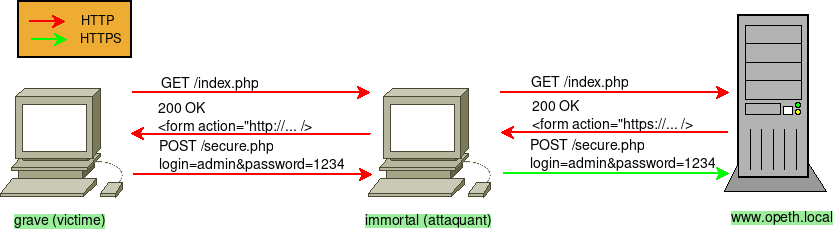
\includegraphics[width=\linewidth]{../medias/sslstrip/attack.png}
\end{frame}

%%%%%%%%%%%%%%%%%%%%%%%%%%%
%  SSLStrip démo          %
%%%%%%%%%%%%%%%%%%%%%%%%%%%

\begin{frame}{Attaque SSLStrip - démonstration}
  % deux images du code source HTML (cf rapport)
  % essayer de mettre des flèches
\end{frame}


\section{SSLStrip+}

\begin{frame}{Fonctionnement de HSTS}
  \begin{exampleblock}{HTTP Strict Transport Security}
    \begin{itemize}
    \item RFC 6797
    \item Entête HTTP 'Strict-Transport-Security'
    \item Date d'expiration
    \end{itemize}
  \end{exampleblock}

  \begin{alertblock}{Problème}
    \begin{itemize}
    \item Ne protège pas la première connexion
    \end{itemize}
  \end{alertblock}

  \begin{block}{Solution}
    \begin{itemize}
    \item HSTS preload
    \end{itemize}
  \end{block}

\end{frame}

\begin{frame}{Attaque SSLStrip+}
  - création d'un faux nom de domaine
  - Ressemblance avec le vrai nom de domaine
  - Remplacement des URL sécurisés par la fausse URL
  - Le navigateur va faire une requête DNS sur le faux domaine
  - L'attaquant doit contrôler la requête
  - SSLStrip peut alors fonctionner
\end{frame}

\begin{frame}{Attaque SSLStrip+}
    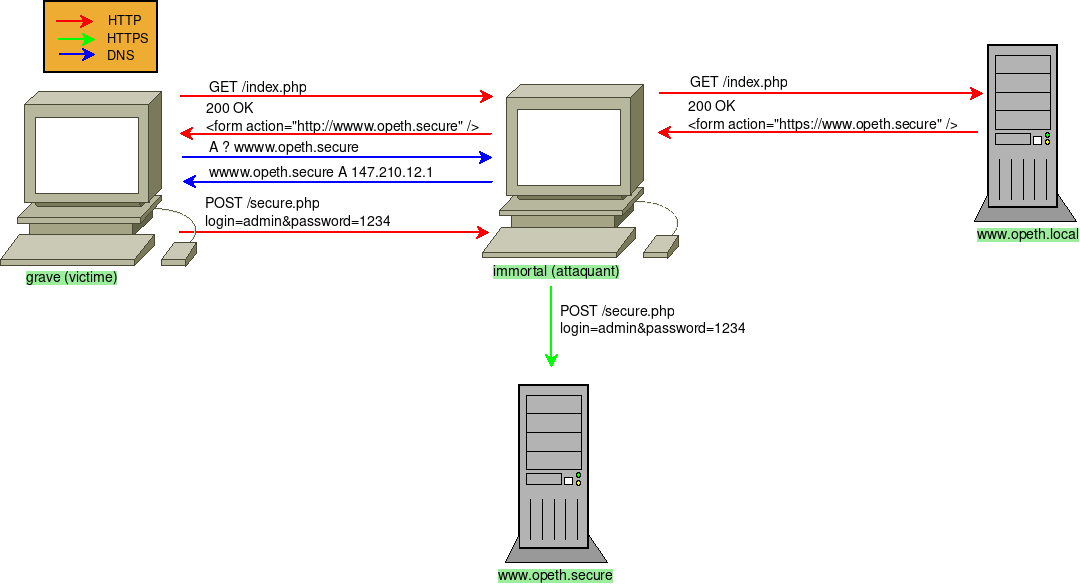
\includegraphics[width=\linewidth]{../medias/sslstrip2/attack.png}
\end{frame}


\section{SSLStrip NTP}

\begin{frame}{Attaque SSLStrip-NTP}

  \begin{block}{Protocole NTP}
    \begin{itemize}
    \item{Synchroniser l'horloge avec un serveur}
    \item{Protocole non-sécurisé}
    \item{Basé sur UDP}
    \end{itemize}
  \end{block}

  \begin{block}{Principes}
    \begin{itemize}
    \item{Attaquer le trafic NTP}
    \item{Expirer l'entrée HSTS}
    \end{itemize}
  \end{block}

  \begin{exampleblock}{Outils}
    \begin{itemize}
    \item{Delorean, ntpd, sntpc}
    \end{itemize}
  \end{exampleblock}

  {\Large \centerline{Retour à SSLStrip...}}
\end{frame}

\begin{frame}{Attaque SSLStrip NTP}
    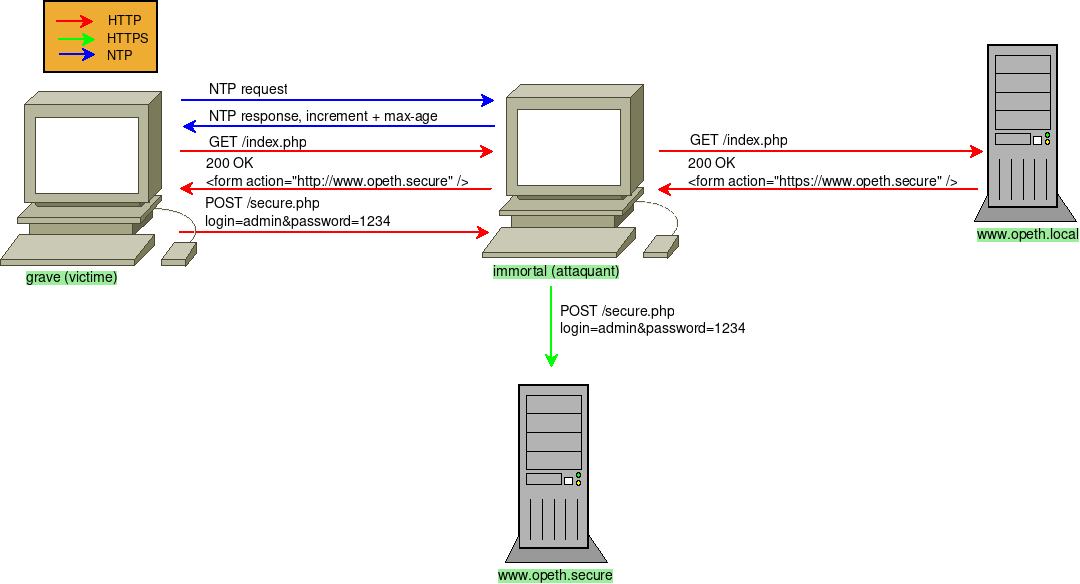
\includegraphics[width=\linewidth]{../medias/sslstrip-ntp/attack.png}
\end{frame}


\section{HTTPS interception}

\begin{frame}{Attaque HTTPS interception}
    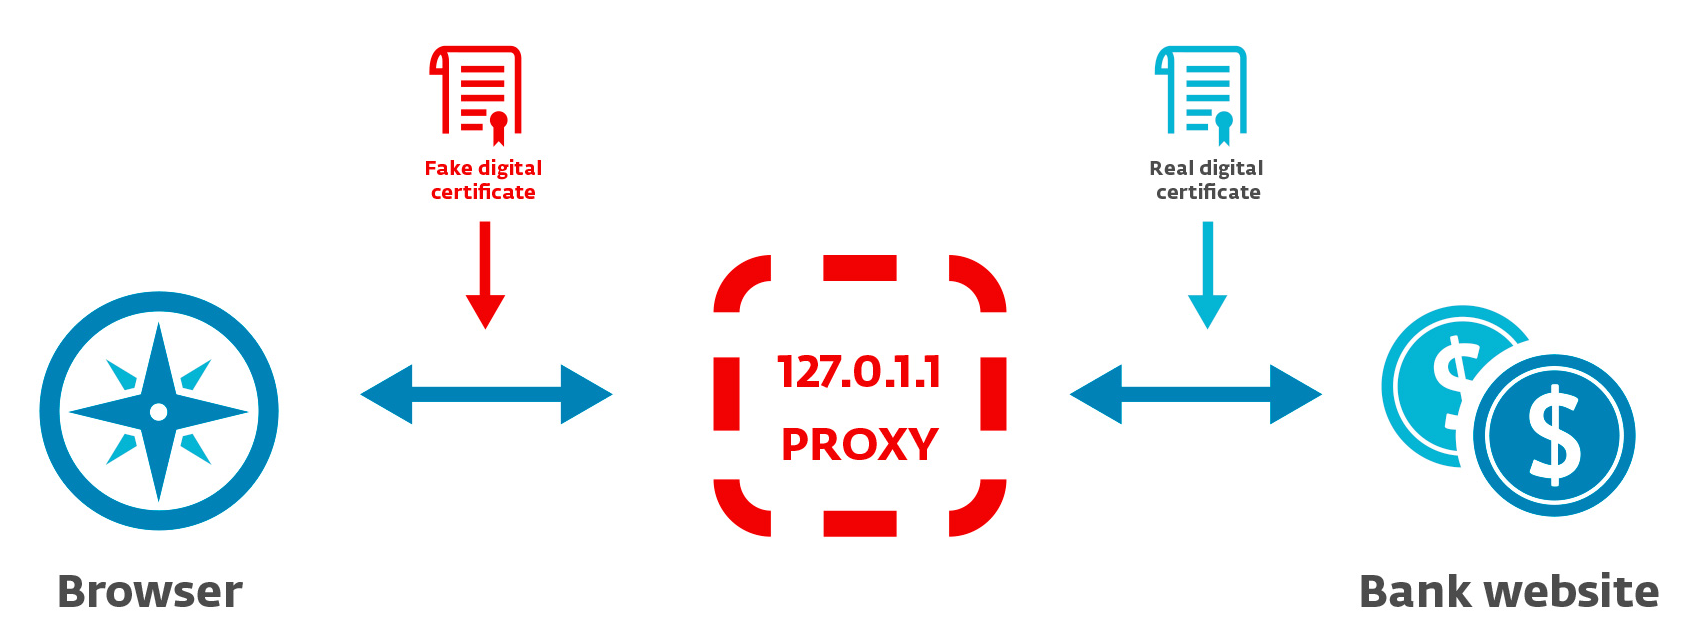
\includegraphics[width=\linewidth]{../medias/interception-https.png}

    \hspace{10cm}

    \begin{columns}
        \begin{column}{0.7\textwidth}
            \begin{block}{Fonctionnement}
                \begin{itemize}
                    \item{Installer un certificat dans le navigateur du client}
                    \item{Faire un proxy https entre client et serveur}
                    \item{Texte en clair entre les deux chiffrements}
                \end{itemize}
            \end{block}

        \end{column}

        \begin{column}{0.3\textwidth}
            \begin{exampleblock}{Scénario}
                \begin{itemize}
                    \item{Entreprise}
                    \item{Antivirus}
                    \item{Attaquant}
                \end{itemize}
            \end{exampleblock}
        \end{column}
    \end{columns}

\end{frame}

\begin{frame}{Attaque HTTPS interception}
    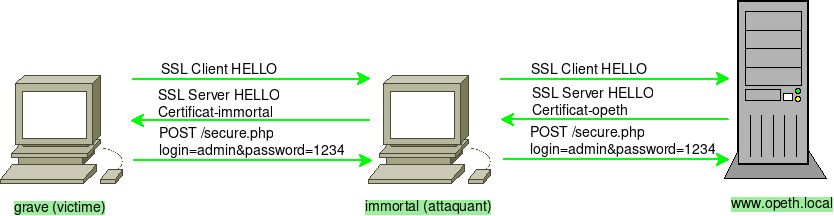
\includegraphics[width=\linewidth]{../medias/https-interception/attack.png}
\end{frame}


\section{Conclusion}
\begin{frame}{Conclusion}
  \begin{block}{Limitations}
    \begin{itemize}
    \item{HTTPS sur \emph{toutes} les pages}
    \item{HTTPS-Interception difficile en pratique}
    \end{itemize}
  \end{block}
  \begin{block}{Contremesures}
    \begin{itemize}
    \item{DANE/TLSA}
    \item{Certificate Transparency}
    \end{itemize}
  \end{block}

  \begin{exampleblock}{Github}
    \begin{itemize}
    \item \url{https://github.com/t00sh/mastercsi-ter/}
    \end{itemize}
  \end{exampleblock}
      { \Large \centerline{Questions ?} }

\end{frame}


\end{document}
